\documentclass{article}

\usepackage[english]{babel}
\usepackage{fancyhdr}

% Write proper math 
\usepackage{amssymb}

% URLS 
\usepackage{hyperref}

% Reference smart
\usepackage{cleveref}

% Font modifiers
\usepackage[utf8]{inputenc}
\usepackage[T1]{fontenc}
\usepackage{fontspec}

% update to modern math font
\usepackage{cmbright}

% titlesec allows us to redefine our headings
\usepackage{titlesec}

% include quotes 
\usepackage{csquotes}

% graphicx for graphics 
\usepackage{tikz}

\usepackage{graphicx}
\graphicspath{ {./gfx/} }

% formatting geometry and paper stuff
\usepackage[
    paper=a4paper,
    % showframe, % debugging
    margin=1.5in]{geometry}% http://ctan.org/pkg/geometry


% !! TESTING 

% \usepackage{blindtext}



%% FONTS SPECIFIED HERE: USE ONE OF THE TWO:

% %% USE PRIMARY FONTS: 
% \setsansfont[
% Extension = .otf ,
% Path=./fnt/primary/ ,
% UprightFont=*-Regular,
% ItalicFont=*-RegularItalic,
% BoldFont=*-Bold,
% BoldItalicFont=*-BoldItalic,
% ]{MessinaSans}

% \setmainfont[
% Extension = .otf ,
% Path=./fnt/primary/ ,
% UprightFont=*-Regular,
% ]{Nantes}


%% USE SECONDARY FONTS (open source): 
% \setsansfont[
% Extension = .ttf ,
% Path=./fnt/secondary/Roboto/ ,
% UprightFont=*-Regular,
% BoldFont=*-Bold,
% ItalicFont=*-Italic,
% BoldItalicFont=*-BoldItalic,
% ]{Roboto}

\setsansfont[
Extension = .ttf ,
Path=./fnt/secondary/Inter/ ,
UprightFont=*-Light,
BoldFont=*-SemiBold,
% BoldFont=*-Regular,
]{Inter}

\setmainfont[
Extension = .otf ,
Path=./fnt/secondary/Noto_Serif_SC/ ,
UprightFont=*-Regular,
BoldFont=*-Bold,
% ItalicFont=*-Italic,
% BoldItalicFont=*-BoldItalic,
]{NotoSerifSC}



% Roboto mono as universal 
\setmonofont[
Extension = .ttf ,
Path=./fnt/ ,
UprightFont=*-Light,
BoldFont=*-Regular,
]{RobotoMono}





% section titles in serif
% \titleformat{\section}{\HUGE\mdseries\rmfamily\leftalign}
% \titleformat{\subsection}{\LARGE\mdseries\rmfamily}
% \titleformat{\subsubsection}{\large\mdseries\rmfamily}
% switch between bfseries and mdseries to get bold face or not
\titleformat*{\section}{\huge\mdseries\rmfamily}
\titleformat*{\subsection}{\Large\mdseries\rmfamily}
\titleformat*{\subsubsection}{\large\mdseries\rmfamily}
\titleformat*{\paragraph}{\normalsize\bfseries\rmfamily} 

% Set main font to be sans serif 
\renewcommand{\familydefault}{\sfdefault}

% PAGE STYLE HEADER AND FOOTER
\setlength{\headheight}{30pt} 
\pagestyle{fancy}
\fancyhf{}
\fancyhead[RE,LO]{ 
\includegraphics[height=30pt]{logo/Corti-Symbol-Black-CMYK.pdf}  }
\fancyhead[LE,RO]{\leftmark}
\cfoot{\thepage}
% \fancyfoot[LE,RO]{\thepage}
% \fancyfoot[LE,RO]{\thepage}



% Start counting sections at 0 
\setcounter{section}{-1}

%%%%%%%%%%%%%%%%%
% Document here %
%%%%%%%%%%%%%%%%%
\begin{document}

\setcounter{page}{0}
\begin{titlepage}
\newgeometry{top=1in,bottom=1in,right=1in,left=1in}
\begin{center}
    % \vspace*{1cm}

    
\includegraphics[width=0.7\textwidth]{logo/Corti-Lockup-Horizontal-Black-CMYK.pdf}
    \vspace{1in}

    \rmfamily
    \huge
    Paper Summaries \\
    \vspace{1cm}
 

    \Large
    Some Joke About VAEs 
    
    \sffamily
    % \vspace{1.5cm}

    \vfill

    \large
    Written @ Corti \\


    \vspace{0.8cm}

    Authors:  \\
    Magnus Berg Sletfjerding \\
    
    \texttt{\{ms\}@corti.ai} \\

    \today \\
    
    \vspace{2cm}


\end{center}
\end{titlepage}

\restoregeometry
\pagenumbering{roman}

\newpage
\vspace*{1cm}
\section*{Abstract}
This was written for me to understand papers in my thesis better. 
Don't be alarmed if you don't understand it 100\%, I probably don't either. 
   
% \newpage
% \tableofcontents

\newpage
\pagenumbering{arabic}
\setcounter{page}{1}

\section{Chapter 0: Auto Encoding Variational Bayes (?)}



\newpage
\section{WaveNet}
The WaveNet paper presents a CNN-based approach to generating audio samples. \cite{oord_wavenet_2016}
Instead of using RNNs as a recurrent architecture, the generative model only conditions on past samples, and as such does not include any hidden "state".

The probability of a waveform \(\mathbf{x}\in \mathbb{R}^T\) is expressed purely as:
\begin{equation}\label{eq:wavenet-probabilities}
    p(\mathbf{x}) = \prod_{t=1}^T  p(x_t | x_1, ..., x_t )
\end{equation}
where $ p(x_t | x_1, ..., x_t ) $ is parametrized only by the \textit{weights} in the network. 


\subsection{Architecture and design}
The WaveNet Architecture draws advantage from three developments: quantized output spaces (as shown in PixelRNN), dilated causal convolutions and gated activation units,

\paragraph{Quantized Output Space with $\mu$ law companding transformation}
Given an audio waveform \(\mathbf{x} \in [-1,1]^T\), transform the audio according to :
\begin{equation}
    f(x_t) = \textrm{sign}(x_t) \frac{ \ln(1 - \mu|x_t|  )}{ \ln(1 + \mu)  }
\end{equation} 
with \(\mu = 255\).


\paragraph{Dilated Causal Convolutions}
A \textit{Causal} Convolution is a fancy way of saying that audio convolutions only work forward in time, not backward.
This is to enforce the forward dependency in \cref{eq:wavenet-probabilities}.

A \textit{Dilated} Convolution is a convolution where the convolution kernel skips over a dimension, increasing the receptive field and observing more of the surrounding environment. 
For an image the simplest dilated convolutional is illustrated in \cref{fig:wavenet-dilated-conv}
\begin{figure}[!ht]
    \begin{small}
        \begin{center}
            \begin{tikzpicture}
                \draw[step=0.5cm,gray,very thin] (-1.45,-1.45) grid (1.95,1.95);

                \fill[blue!40!white] (-1,-1) rectangle (1.5,1.5);
                \fill[white] (-0.5,-0.5) rectangle (1,1);
                \fill[blue!40!white] (0,0) rectangle (0.5,0.5);

            \end{tikzpicture}
        \end{center}
        \caption{A Simple Pixel Dilated Convolution}
        \label{fig:wavenet-dilated-conv}
    \end{small}
\end{figure}

Accordingly, for an audio signal, it would look like what we see in \cref{fig:wavenet-dilated-causal-conv}



\begin{figure}
    \begin{small}
        \begin{center}
            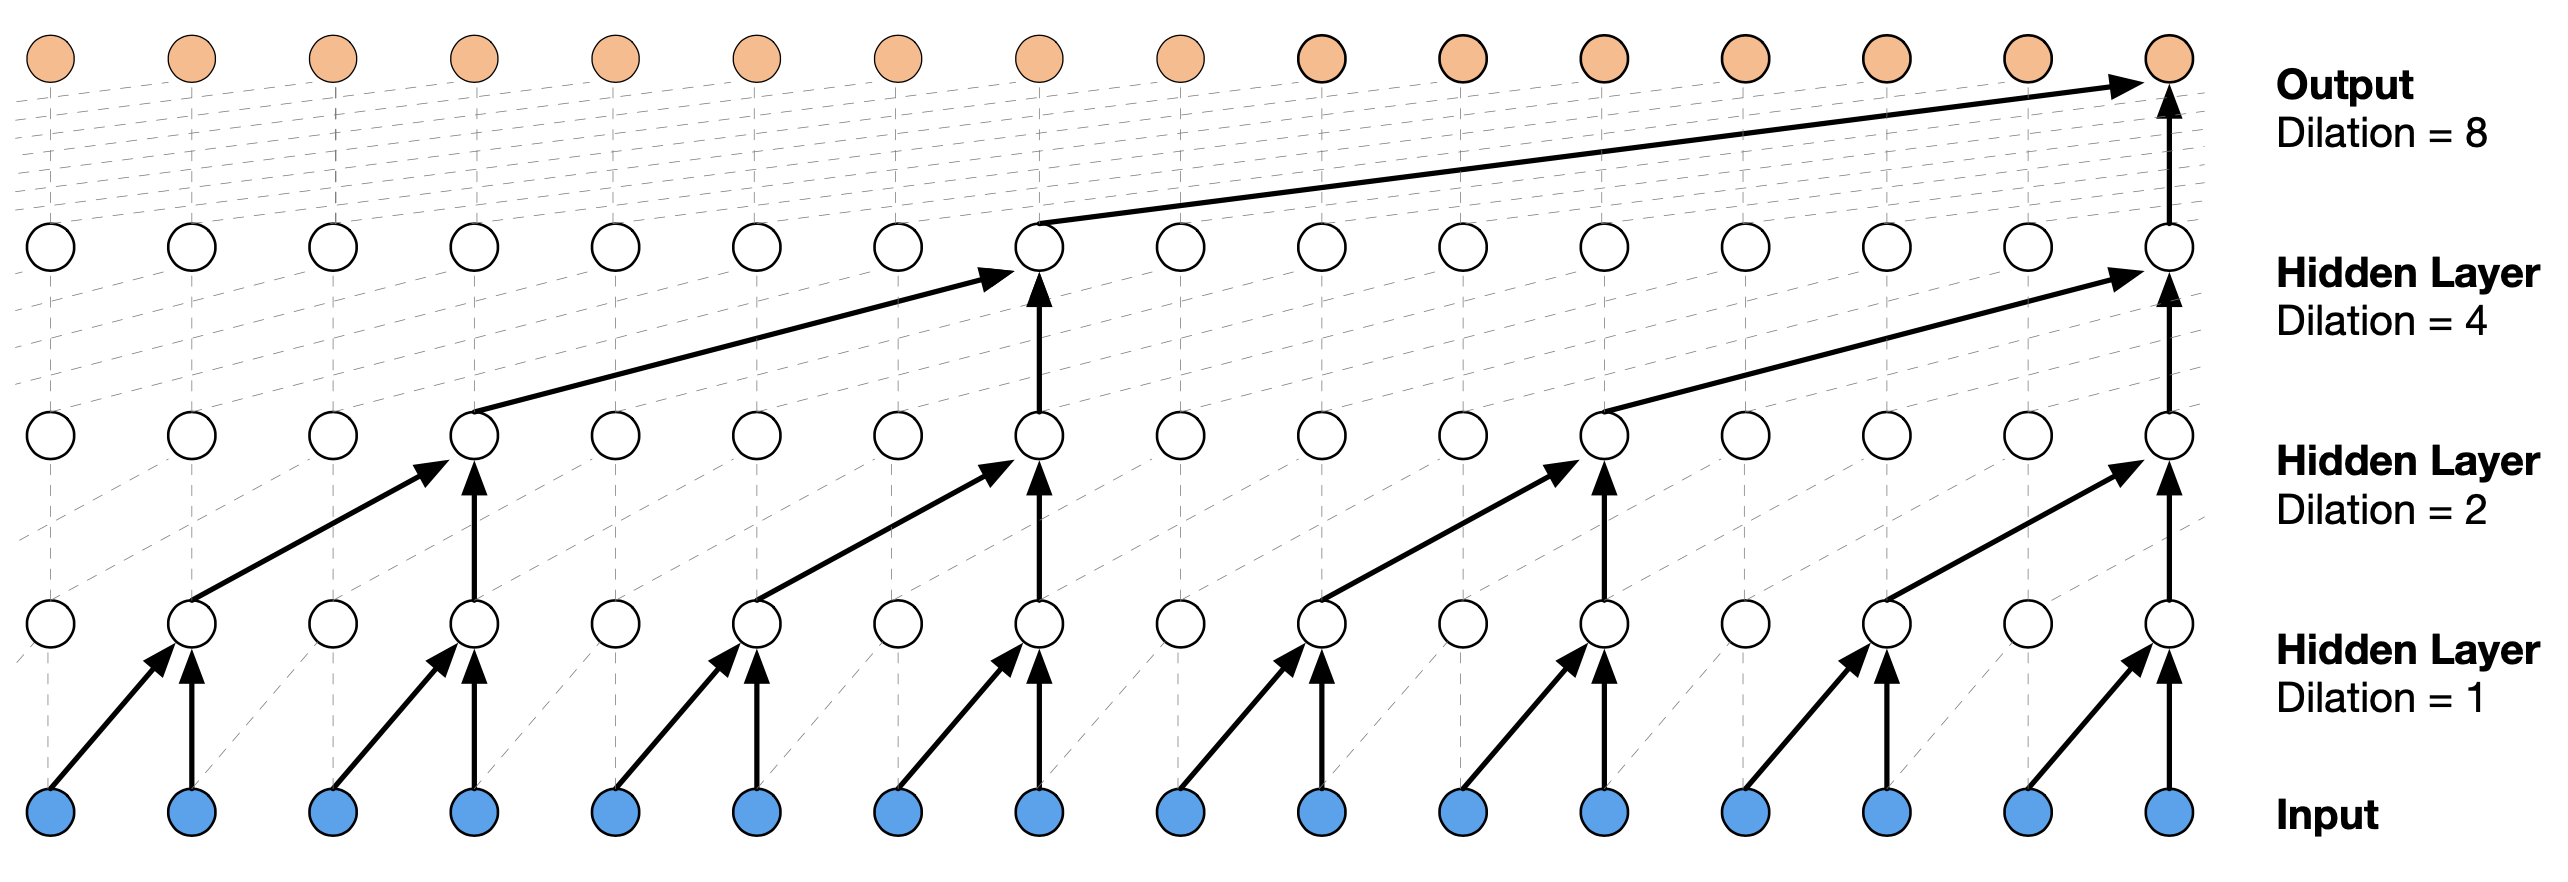
\includegraphics[width=0.95\textwidth]{figures/wavenet-dilated-causal-conv.png}
        \end{center}
        \caption{The Dilated Causal Convolution in WaveNet} 
        \label{fig:wavenet-dilated-causal-conv}
    \end{small}
\end{figure}



\paragraph{Gated Activation Units}
Each Convolution layer, Insteadof \textit{just} having a filter weight, also has a \textbf{gating weight}.
Hence the weights \(\mathbf{W} \in \mathbb{R}^{K \times 2} \), with \(K\) as the number of layers. 
The operation of layer $k \in [0, K]$, is parametrized as: 

\begin{equation}
    \mathbf{z} = \tanh ( \mathbf{x} * W_{k, f} ) \odot \sigma ( \mathbf{x} * W_{k, g} )
    \label{eq:wavenet-gated-activation}
\end{equation}





\paragraph{Summary of architechture}
The architecture is summed up in \cref{fig:wavenet-architecture}.
It's important to note that the Causal Convolution setup as described in \cref{fig:wavenet-dilated-causal-conv} only is applied \textit{once}, as the first layer.
This makes the entire rest of the network a simple convolutional network with dilation, as the \textbf{first (causal) convolutional stack ensures that the rest of the network will only see samples from the past.}
In all other respects we can consider this a standard CNN architecture. 


\begin{figure}
    \begin{small}
        \begin{center}
            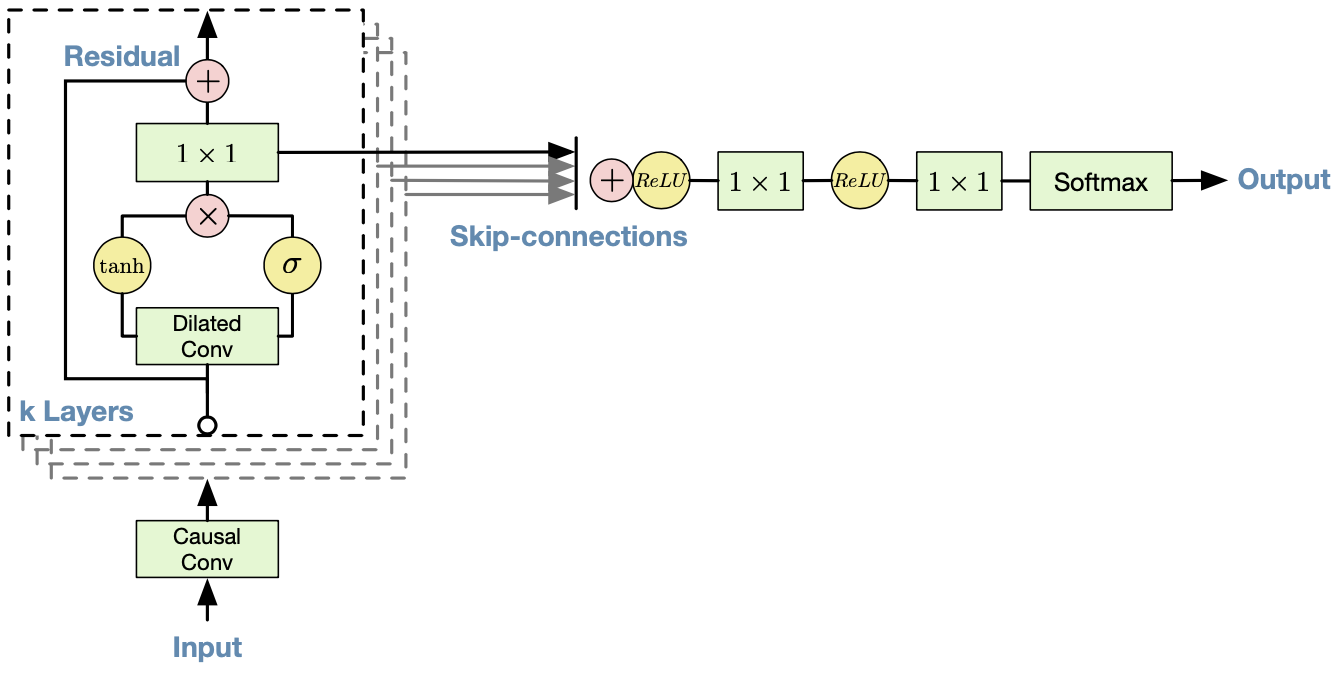
\includegraphics[width=0.95\textwidth]{figures/wavenet-architecture.png}
        \end{center}
        \caption{Overall Residual Architecture of WaveNet. 
        Skip connections happen from \textit{every Convolutional Layer} to the final softmax.}
        \label{fig:wavenet-architecture}
    \end{small}
\end{figure}


\subsubsection{Extending architecture to include latent representations of speaker}
It's possible to add a latent representation \(\mathbf{h}\), extending \cref{eq:wavenet-probabilities} to:

\begin{equation}\label{eq:wavenet-probabilities-ext}
    p(\mathbf{x}|\mathbf{h}) = \prod_{t=1}^T  p(x_t | x_1, ..., x_t, \mathbf{h} )
\end{equation}

There are two ways to represent this:

\paragraph{Global Conditioning (Speaker, Accent, Noise level)}
Here we set \(\mathbf{h}\) to a single global latent, representing a constant over the entire sequence. 
The activation from \cref{eq:wavenet-gated-activation} then becomes

\begin{equation}
    \mathbf{z} = \tanh ( \mathbf{x} * W_{k, f} + V^T_{k, f}\mathbf{h}) \odot \sigma ( \mathbf{x} * W_{k, g} + V^T_{k, g}\mathbf{h})
\end{equation}
With \(V_{k, *}\) is a linear projection , and the resulting vector \(V^T_{k, f}\mathbf{h}\) is broadcast over time \(T\).


\paragraph{Local Conditioning (Tone of voice, changing noise levels over the call}
Here we define \(h_t\), and use a ConvNet to upsample \(h_t\) to \(\mathbf{y} = f(\mathbf{h})\), so \cref{eq:wavenet-gated-activation} becomes:

\begin{equation}
    \mathbf{z} = \tanh ( \mathbf{x} * W_{k, f} + V_{k, f}*\mathbf{y}) \odot \sigma ( \mathbf{x} * W_{k, g} + V_{k, g}*\mathbf{y})
\end{equation}

\subsection{Results}

The main results here are evaluated on "subjective naturalness" by human evaluators. 
As such, WaveNets have outperformed previos TTS methods.
That's not really that interesting but it makes for a cool listen: \href{https://deepmind.com/blog/article/wavenet-generative-model-raw-audio}{here}

\newpage
\section{Paper 2: Vector Quantized VAE (VQ-VAE)}
Title:  \textit{Neural Discrete Representation Learning} \cite{oord_neural_2018}.
\\



Main points: 
\begin{itemize}
    \item Avoiding Posterior Collapse
    \item Discrete Latent
    \item With the right prior, generates speech/audio well  % TODO: elaborat
    \item Language Learning through raw speech
    \item Speaker Conversion
\end{itemize}


The main point of the VQ-VAE lies in that it uses a discrete (i.e. \textit{categorical}) embedding space as its latent space. 


\subsection{Model Components and Architecture}
The model is described in \cref{fig:vqvae-arch}.
What's very important to realize is that \textbf{the VQ-VAE is deterministic, not stochastic!}

\subsection{Discrete Latent Embedding Space}
The VQ VAE uses a \(D\)-dimensional latent space with \(K\) embedding vectors.
This means that the latent space \textbf{does not sample from a latent space} (so it's not a real VAE) but instead \textbf{does a nearest-neighbor embedding lookup}. 
We define the embedding vectors as 
\[
  e_i \in \mathbb{R}^D, i \in \{1 .. K\}, \therefore e \in \mathbb{R}^{K \times D}
\]

\begin{figure}[ht]
    \begin{small}
        \begin{center}
            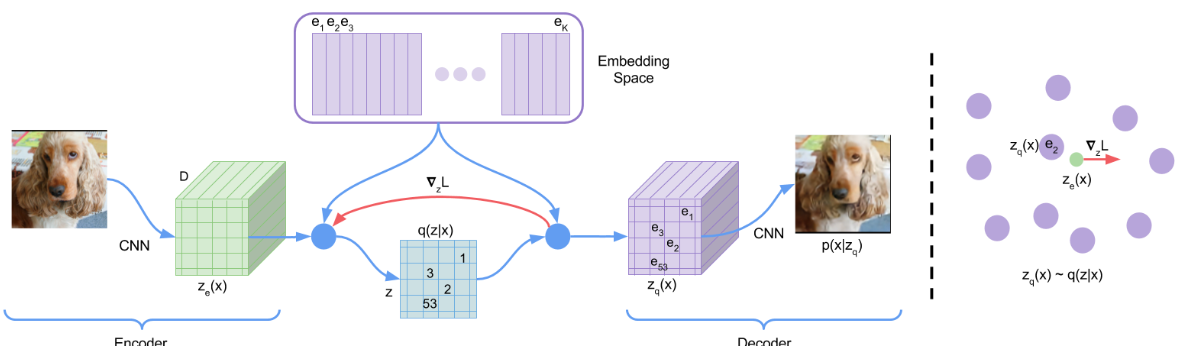
\includegraphics[width=0.95\textwidth]{figures/vqvae-arch}
        \end{center}
        \caption{VQ-VAE Architecture. 
        Right: Embedding space. 
        Left: Overall Architecture. 
        Note that the CNN works as a down/upsampling CNN, so as to avoid identity operations all the way through. 
        }
        \label{fig:vqvae-arch}
    \end{small}
\end{figure}

\subsection{Loss function}

The loss function \cref{eq:vqvae-loss} is composed of 3 parts, here covered in detail:

\begin{equation}
    L = 
    \log p(x| z_q(x)) + 
    || \mathrm{sg}[z_e (x) ] - e ||_2^2 + 
    || z_e (x)  - \mathrm{sg}[e] ||_2^2
    \label{eq:vqvae-loss}
\end{equation}

We denote \(z_e(x)\) as the \textbf{encoder output} and \(z_q(x)\) as the \textbf{quantized encoding.} 
We also use \(\mathrm{sg}\) to denote the stopgradient operator (identity function forward but 0 partial derivatives).

\paragraph{Reconstruction Loss}
\[
    \log p(x| z_q(x)) +     
\]
This refers to the probability of the data \(x\) given the embedding \(z_q(x)\).

The reconstruction loss is optimized by the \textbf{encoder} and \textbf{decoder}.

\paragraph{Embedding Loss}
\[
    || \mathrm{sg}[z_e (x) ] - e ||_2^2 
\]

The embedding loss quantifies \textit{how far away from the samples the embeddings are.}
This loss comes from Vector Quantization (VQ), a dictionary learning algorithm. 
The VQ objective seen here moves the \textit{discretized} embedding vectors \(e_i \in \mathbb{R}^D\) towards the \textit{continuous encoder outputs} \(z_e(x)\).
This means that the model is able to learn embeddings and update them at need. 

The embedding loss is optimized by the \textbf{embedding}.

\paragraph{Commitment Loss}
\[
    || z_e (x)  - \mathrm{sg}[e] ||_2^2
\]
The commitment loss quantifies \textit{how far away from the embeddings a sample is.}
The embedding space is dimensionless in volume, and therefore the output of the encoder can grow arbitrarily large, while embeddings can't keep up. 
This equates to the encoder seeing an out-of-distribution sample and encoding it as very far away from the latent space embeddings. 

The commitment loss is optimized by the \textbf{encoder}.



\subsection{Experiments and Results}

\subsubsection{Images}
Downsampling from \(128 \times 128 \times 3 \) to a \( 32 \times 32 \times 1 \) discretized latent space on the ImageNet ( \(128 \times 128 \times 3\) ) dataset.

For images, the encoder/decoder is the PixelCNN. 



\subsubsection{Audio}
For audio, the VQ-VAE is trained on the VCTK dataset, which has 109 different speakers. 
The encoder is \textbf{6 strided convolutions with stride 2 and window-size 4}, corresponding to a downsampling of 64x. 
The latent space is a single 512-dimensional discretized space. 
In addition to the latent space, the decoder is conditioned on a 1-hot speaker embedding. 

\paragraph{Results}
The VQ-VAE manages to learn to interchange speakers very well. To cite the paper:

\begin{displayquote}
    This means that the VQ-VAE has, without any form of linguistic supervision, 
    learned a high-level abstract space that is invariant to low-level features and only encodes the content of the speech.
\end{displayquote}


The authors also ran an experiment where they mapped a 128-dimensional discrete latent space to 41 phonemes. 
Using this simple mapping they found the accuracy to be \(49.3\%\), without further mappings. 



\newpage
\section{Clockwork Variational Autoencoders}
\paragraph{Authors} Vaibhav Saxena, Jimmy Ba, Danijar Hafner. \cite{saxena_clockwork_2021}

The clockwork VAE aims to learn higher-level, abstract prediction timelines \textit{without needing to predict the actual images going forward.}
They term this "Temporally Abstract Latent Dynamics Models".


\subsection{CW-VAE Architecture and components}
The CW-VAE is composed of a hierarchy of "states" as seen in \cref{fig:cwvae-architecture}

\begin{figure}[hb]
    \begin{small}
        \begin{center}
            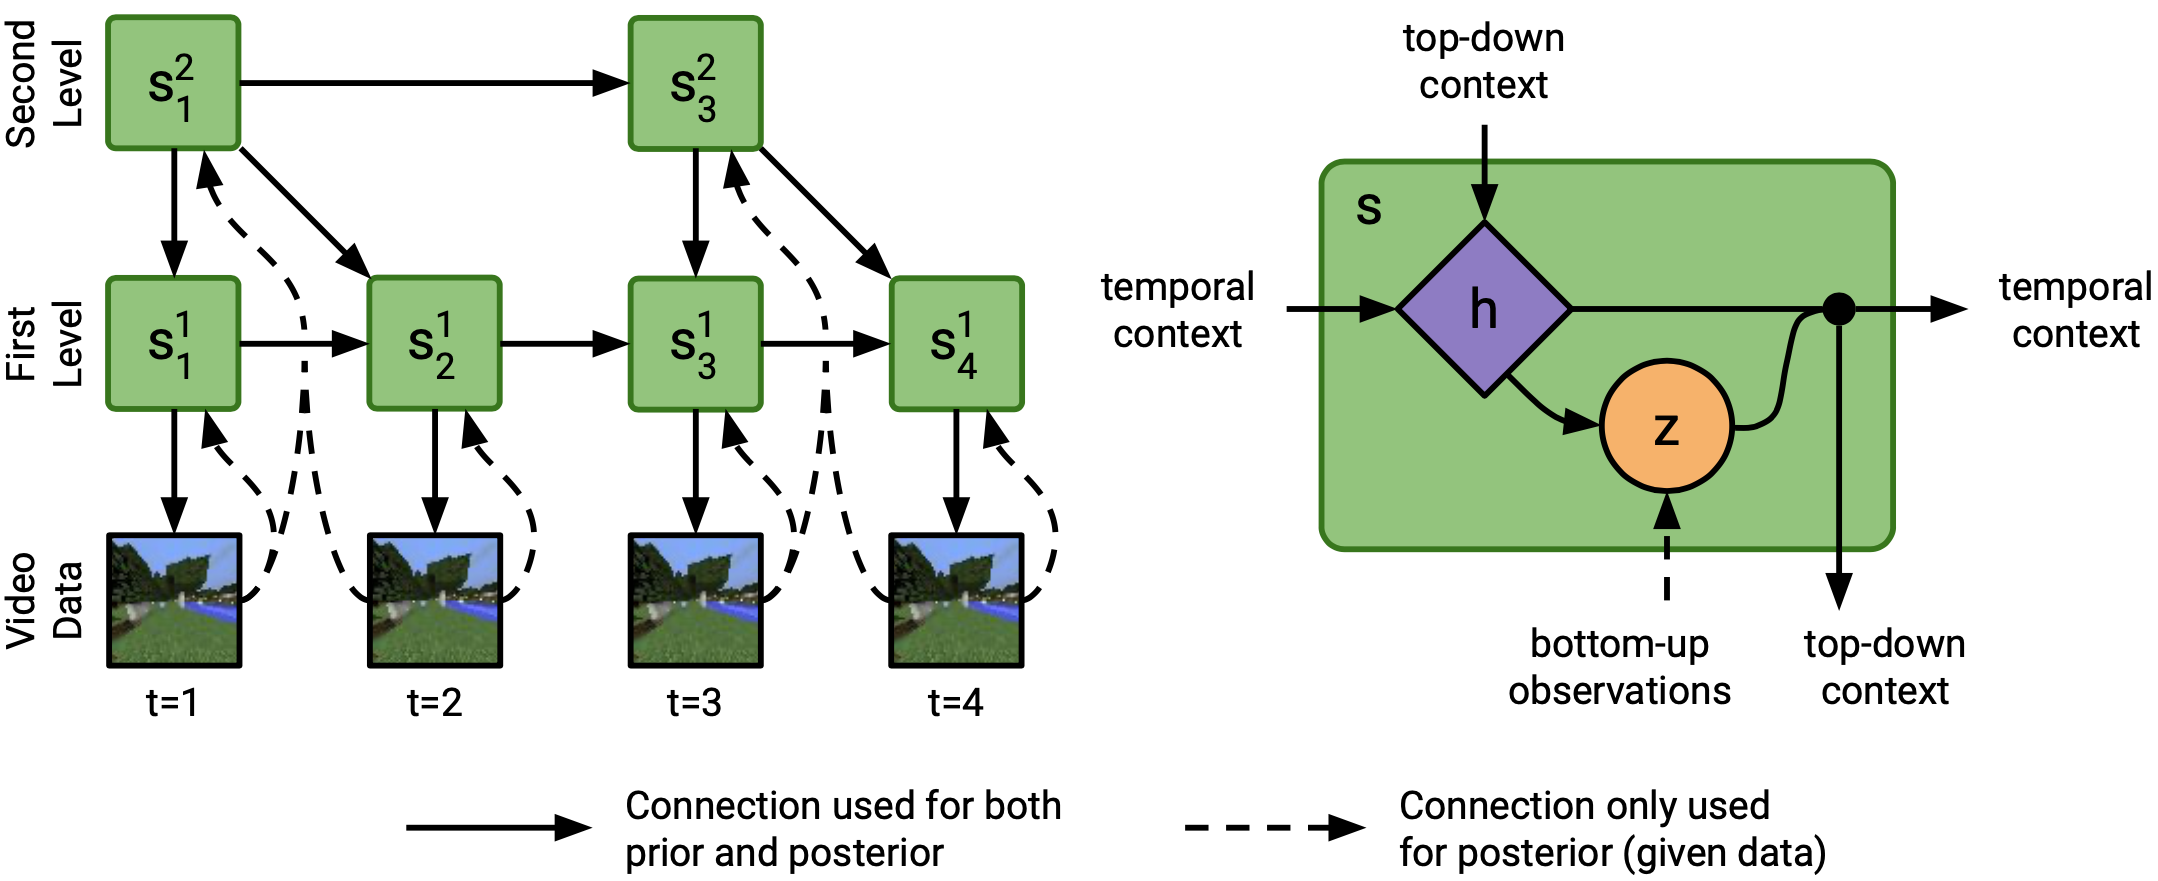
\includegraphics[width=0.95\textwidth]{figures/cwvae-architecture.png}
        \end{center}
        \caption{
            \textbf{Arrows:} Solid is the generative model, dashed is the inference model. 
            \textbf{Left:} The general setup of the CW-VAE, with a temporal abstraction factor \(k=2\). 
            The upper state only updates every kth timestep, and this would compound in higher hierarchies. 
            As such we see that the video frame with \(t=2\) still will feed into \(s^2_1\), and likewise the frame at \(t=4\) feeds into \(s^2_3\)
            \textbf{Right:} The internals of states \(s_l^t\). 
            }
        \label{fig:cwvae-architecture}
    \end{small}
\end{figure}

\subsubsection{The latent states \(s^l_t\)}

The latent state is composed of a deterministic variable \(h_t\) and a stochastic variable \(z_t\). 


\paragraph{Updates to latent states during inference}
The latent states are updated at the "active" timesteps 
\(\mathcal{T}_l = \{ t \in [1, T] | t \mathrm{mod} k^{l-1} = 1 \}\), 
where \(k\) is the dilation factor.
This means that latent states will only be updated at each \(k_{l-1}\) timestep, where \(l\) is the "level" of the latent variable.
Otherwise, the states are copied from the previous timestep.

During inference, all "active" latents will receive a CNN image embedding (in \cref{fig:cwvae-architecture} this is the "bottom-up observations").
The posterior \(q^l_t\) for that latent is calculated 
"as a function (what function?) of the input features, 
\hl{(ASK JAKOB: Is this the arrow from $z$ to the combination node?) } 
the posterior sample at the previous step (temporal context), 
and the posterior sample above (top-down context)"
The posterior / "Gaussian Belief" \(q^l_t\), which is a diagonal Gaussians with means and variances predicted from the deterministic variable.


The deteministic variable is updated with a GRU at every active step.

\subsubsection{Embeddings and layers in between.}

The authors (Appendix C) claim to have used "architectures very similar to the DCGAN".

The DCGAN paper's decoder architecture is shown in \cref{fig:cwvae-dcgan-arch}. \cite{radford_unsupervised_2016}

\begin{figure}[hb]
    \begin{small}
        \begin{center}
            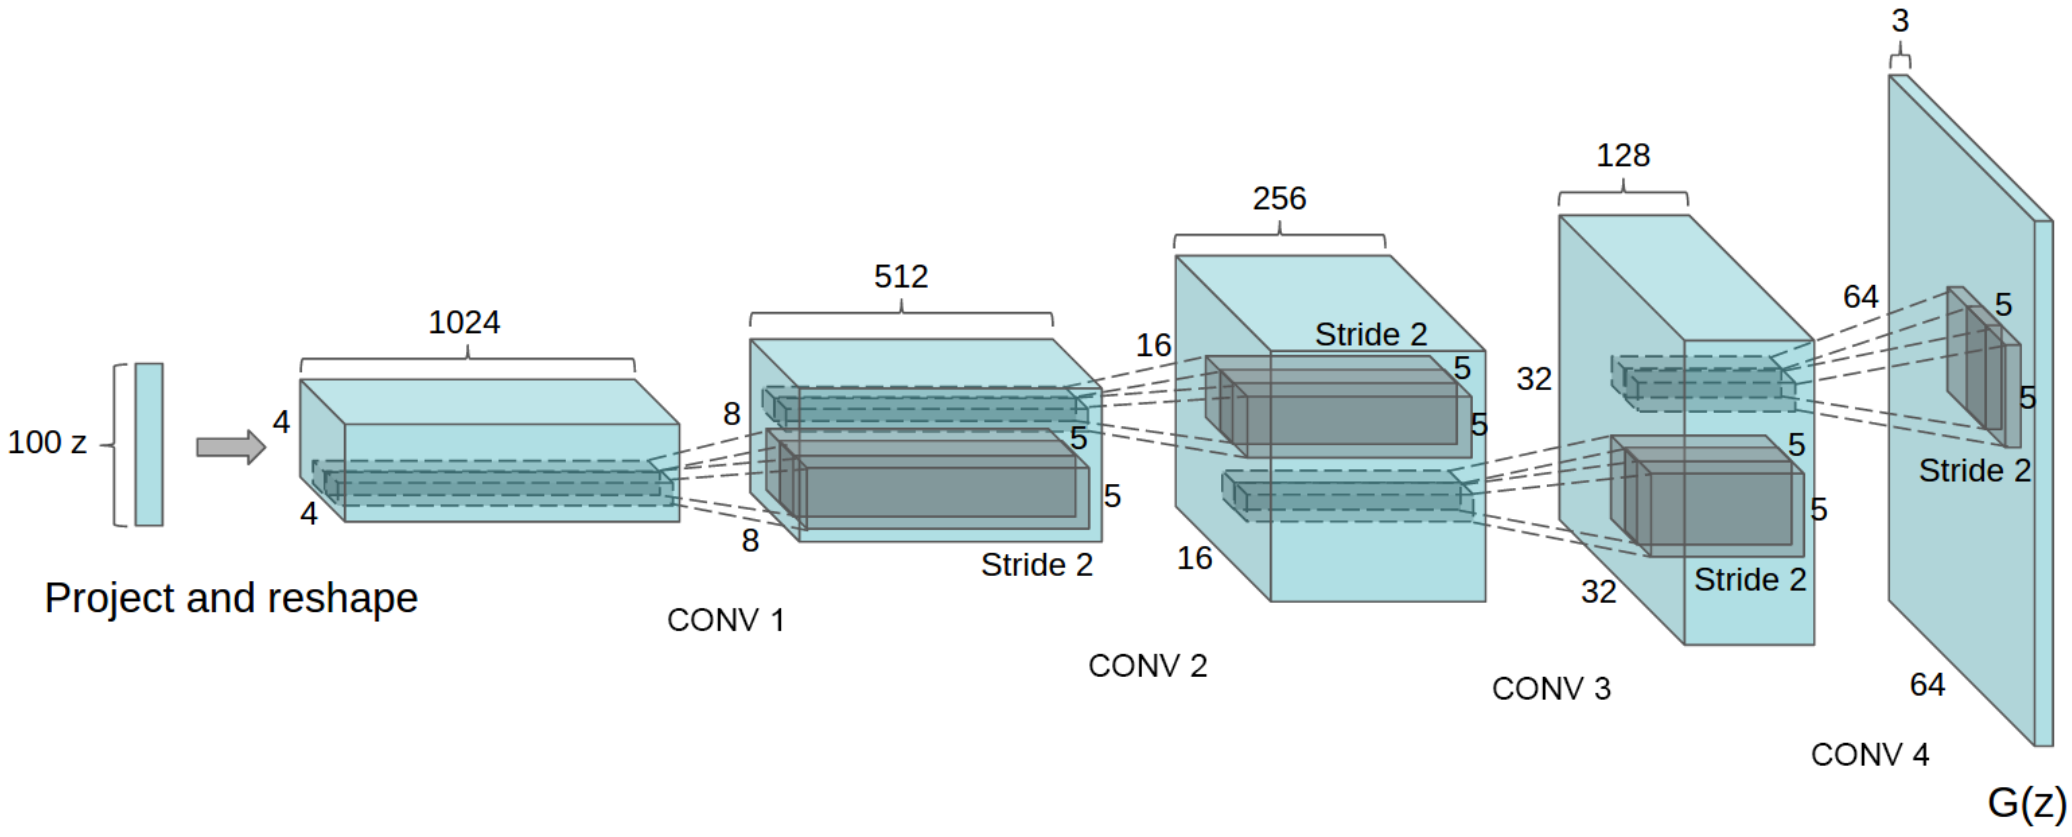
\includegraphics[width=0.95\textwidth]{figures/cwvae-dcgan-arch.png}
        \end{center}
        \caption{\textit{From DCGAN paper: }
        A 100 dimensional uniform distribution Z is projected to a small spatial extent convolutional representation with many feature maps.
        A series of four fractionally-strided convolutions (in some recent papers, these are wrongly called
        deconvolutions) then convert this high level representation into a 64 × 64 pixel image. Notably, no
        fully connected or pooling layers are used.}
        \label{fig:cwvae-dcgan-arch}
    \end{small}
\end{figure}



\subsection{General Comments} % (fold)
The CWVAE paper manages to show very promising results in terms of temporal abstraction. 
They also conjecture that they would be able to do similar things with "more data more GPU" but that we lack good validation metrics. 


NB This paper has a good appendix to keep in mind. 

% subsection General Comments (end)


\newpage
\section{Chapter 4: }


% \newpage


\bibliographystyle{abbrv}
\bibliography{vae}

\end{document}
